
%(BEGIN_QUESTION)
% Copyright 2015, Tony R. Kuphaldt, released under the Creative Commons Attribution License (v 1.0)
% This means you may do almost anything with this work of mine, so long as you give me proper credit

In the following baffle/nozzle system, the nozzle pressure is allowed to react against any external force by generating a force with a bellows unit, to push the baffle away from the nozzle.  The particular bellows in this mechanism is designed to be ``slack,'' having little spring effect to self-restrain its motion.  Whatever force generated by the pressure acting against the bellows' surface area gets directly transferred to the lever:

$$\includegraphics[width=15.5cm]{i00200x01.eps}$$

What will happen in this system if someone pushes the lever toward the nozzle with their thumb?  Explain every step in your reasoning -- don't just describe a final result!

\vskip 10pt

Now, suppose we modify this system to have a bellows with a larger diameter:

$$\includegraphics[width=15.5cm]{i00200x02.eps}$$

What will happen in this system if someone pushes the lever toward the nozzle with the same amount of force as before (with the smaller bellows)?  How will this system respond to the same stimulus?  Again, explain every step in your reasoning -- don't just describe a final result!

\vskip 10pt

\filbreak

What will happen in this system if we were to take the original (smaller) bellows mechanism and push on it with the same force but at a position closer to the pivot point than the bellows?  As usual, explain every step in your reasoning:

$$\includegraphics[width=15.5cm]{i00200x03.eps}$$



\vskip 20pt \vbox{\hrule \hbox{\strut \vrule{} {\bf Suggestions for Socratic discussion} \vrule} \hrule}

\begin{itemize}
\item{} Explain, in simple terms, what effect bellows size has on the {\it gain} of the system, and why.
\item{} Suppose the compressed air supply pressure was 10 PSI in both cases.  If this supply pressure were to drop to a lower value such as 8 PSI, what effect (if any) would this have on the gauge pressure in each scenario as the system responds to the same amount of applied force?  Why or why not?
\item{} Determine whether or not the output pressure would rise to the same level with force applied to the lever if the air supply was cut off (and the supply tube plugged so that air could not leak out).
\item{} A common misconception among students first analyzing these mechanisms is that the output pressure is being generated by the bellows: that is to say, that the action of {\it collapsing} the bellows by the force of the hand is what makes the air inside become compressed.  Explain why this is a misconception, and further explain how and why the resulting pressure arises.
\end{itemize}


\underbar{file i00200}
%(END_QUESTION)





%(BEGIN_ANSWER)

The system with the 0.75 square inch bellows unit will respond to the 1.2 pound force by generating a nozzle pressure of 1.6 PSI.  The baffle will hardly move at all: perhaps only $1 \over 1000$ of an inch!

\vskip 10pt

With a larger bellows in place, the system becomes less sensitive.  The nozzle pressure indicated by the gauge will be {\it less} for the same amount of hand force (only 0.8 PSI instead of 1.6 PSI).  Another way to say this is that the {\it gain} of this pneumatic system is less with a larger bellows.  Once again, the baffle will hardly move at all.

\vskip 10pt

With the smaller bellows at work, and the force applied at the mid-point of the lever, the pressure will be 0.8 PSI because the bellows will only have to exert 0.6 pounds of force to balance the applied 1.2 pounds at the mid-point.  Here, we see a different way to achieve a reduced gain that does not require a new bellows size.

%(END_ANSWER)





%(BEGIN_NOTES)


%INDEX% Basics, pneumatics: force-balance mechanism

%(END_NOTES)


